		\tikzset{line/.style={-latex}} 
		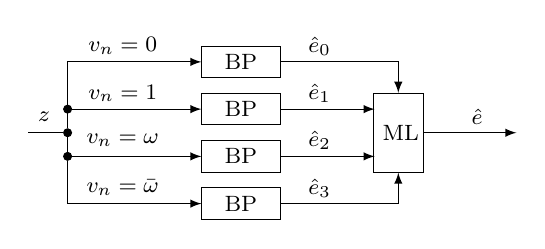
\begin{tikzpicture}
    \node[draw=none] at (0,3.2) {\footnotesize$\bm{z} $};
    \node[draw,circle,fill,inner sep=1pt] at (0.3,3)(s) {};
    \node[draw,circle,fill,inner sep=1pt] at (0.3,3.3) (s1){};
    \node[draw,circle,fill,inner sep=1pt] at (0.3,2.7) (s2) {};

    \draw[] (-0.2,3) -- (s);
    
    \draw[] (2,3.7) rectangle ++(1,0.4);
    \node[draw=none] at (1,4.1) {\footnotesize $v_n=0$};
    \node[draw=none] at (2.5,3.9)(BP1) {\footnotesize BP};  
    \draw[line] (s1) |- (2,3.9);
    
    \draw[] (2,3.1) rectangle ++(1,0.4);
    \node[draw=none] at (1,3.5) {\footnotesize $v_n=1$};
    \node[draw=none] at (2.5,3.3)(BP2) {\footnotesize BP};
    \draw[line] (s) |- (2,3.3);
    
    \draw[] (2,2.5) rectangle ++(1,0.4);
    \node[draw=none] at (1,2.9) {\footnotesize $v_n=\omega$};
    \node[draw=none] at (2.5,2.7)(BP3) {\footnotesize BP};
    \draw[line] (s) |- (2,2.7);
    \draw[] (2,1.9) rectangle ++(1,0.4);
    \node[draw=none] at (1,2.3) {\footnotesize $v_n=\bar{\omega}$};
    \node[draw=none] at (2.5,2.1)(BP4) {\footnotesize BP};
    \draw[line] (s2) |- (2,2.1);

    \node[draw,rectangle,text width=0.4cm, minimum height=1cm,align=center] at (4.5,3)(w) {\footnotesize ML};

    \node[draw=none] at (3.5,4.1) {\footnotesize $\hat{\bm{e}}_0$};
    \node[draw=none] at (3.5,3.5) {\footnotesize $\hat{\bm{e}}_1$};
    \node[draw=none] at (3.5,2.9) {\footnotesize $\hat{\bm{e}}_2$};
    \node[draw=none] at (3.5,2.3) {\footnotesize $\hat{\bm{e}}_3$};

    \draw[line] (3,3.9) -| (w);
    \draw[line] (3,3.3) -- (4.2,3.3);
    \draw[line] (3,2.7) -- (4.2,2.7);
    \draw[line] (3,2.1) -| (w);
    
     \node[draw=none] at (5.5,3.2) {\footnotesize$\hat{\bm{e}}$};
     \draw[line] (w) -- (6,3);
     \end{tikzpicture}